\section{Bestimmung des hadronischen Wirkungsquerschnitts $\sigma_0^{Had}$}
\subsection{Selektion der hadronischen Ereignisse}
Wir haben mehrere Datensamples zu Verfügung gehabt. Zunächst waren dort die gemessenen L3-Daten, die bei verschiedenen Schwerpunktenergien $\sqrt{s}$ aufgenommen wurden (bei 89.48 GeV, 91.33 GeV und 93.02 GeV). Die integrierten Luminositäten unterscheiden sich auch und wurden in \cite[S.9]{script} gegeben; außerdem konnten wir mit zwei Monte-Carlo-Datensätzen (MC) arbeiten, die uns die der aktuellen Theorie entsprechende Verteilungen von Hadronen und Myonen gab. Mit diesen Simulationsdaten konnten wir überprüfen, welche Wirkung unsere Cuts auf den jeweiligen $Z^0$-Zerfallskanal hatten. So konnten wir feststellen, dass bei hadronischen Ereignissen immer mindestens ca. 9 Cluster (separierte Einträge im Kalorimeter) Teilchen detektiert wurden (siehe \fref{Ncluster_vgl}).
\begin{figure}[htb]
	\centering
	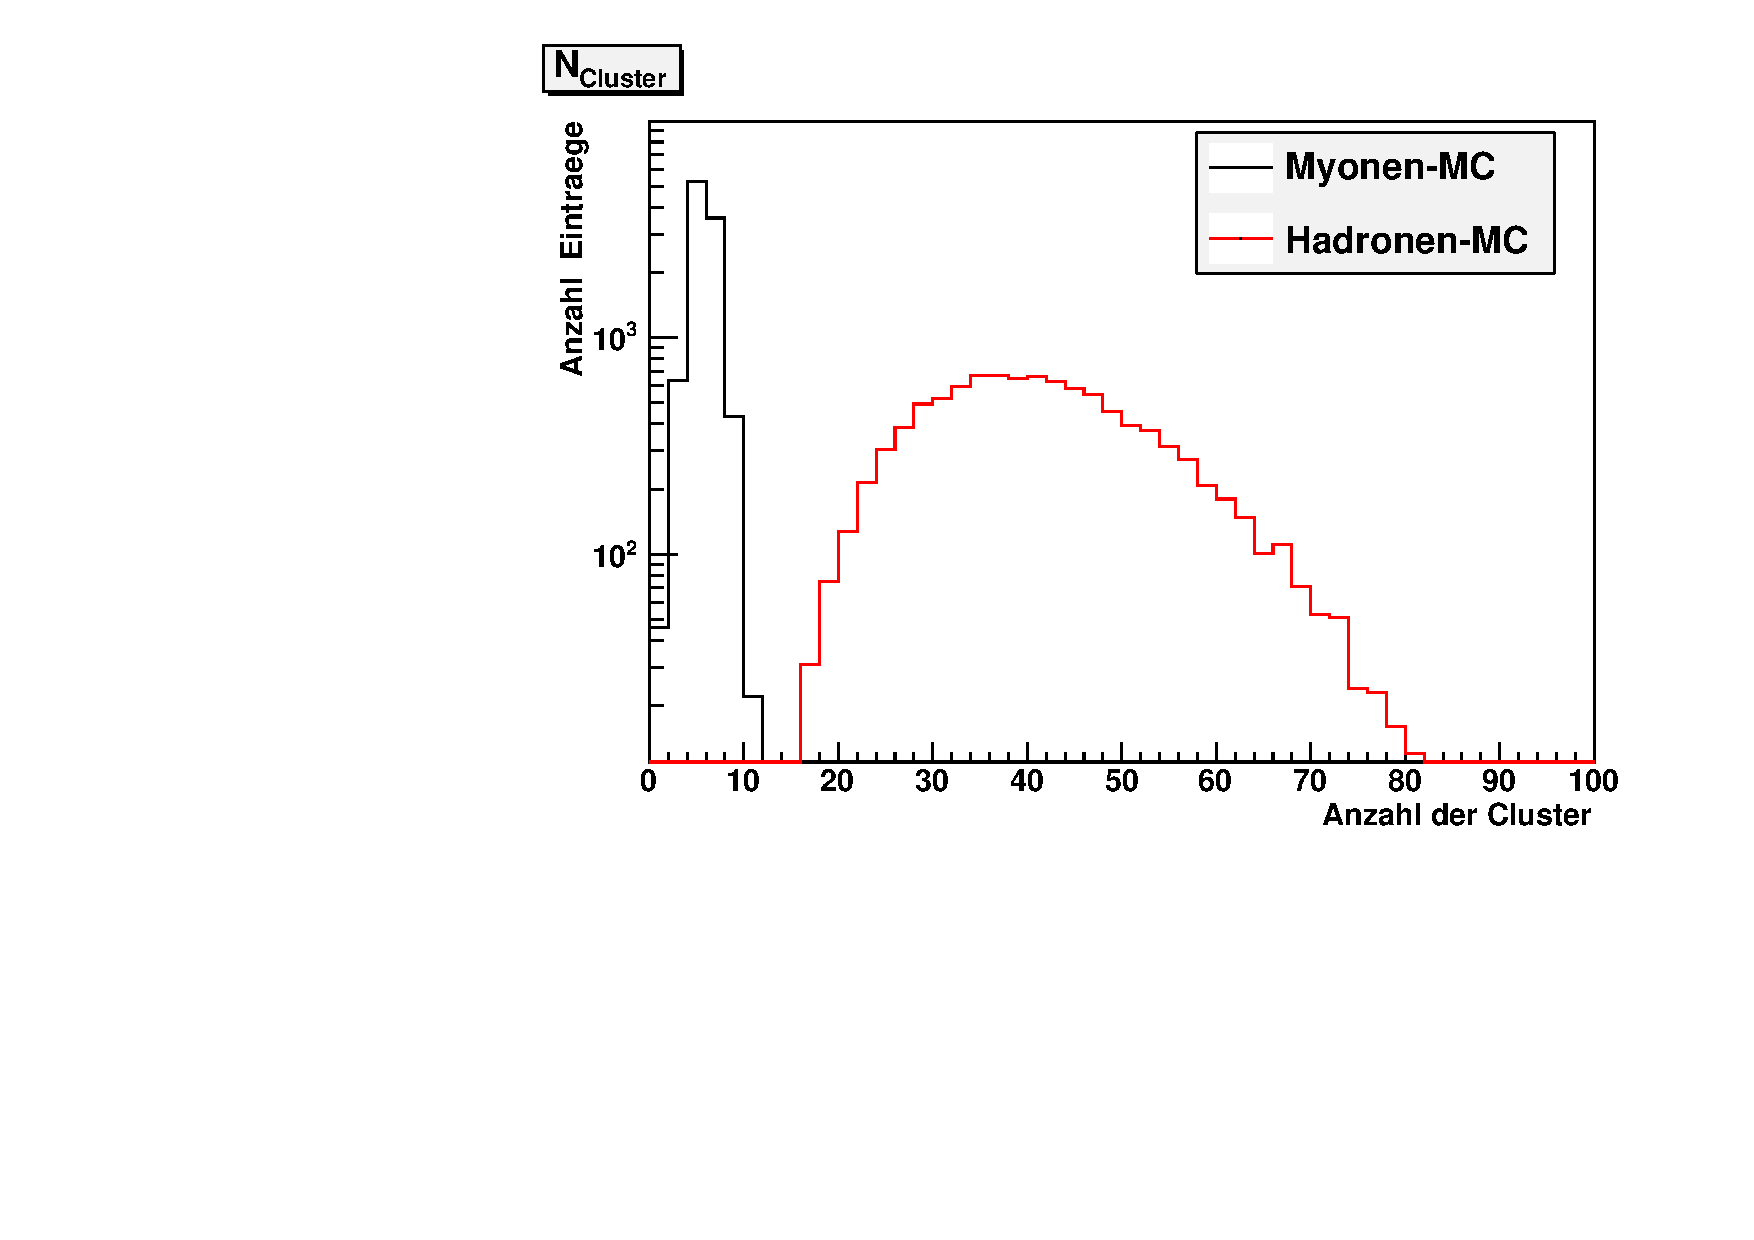
\includegraphics[width=1\columnwidth,keepaspectratio]{Ncluster_vgl.pdf}
	\caption{Verteilung der Kalorimetereinträge für MC-Samples}
	\label{fig:Ncluster_vgl}
\end{figure}
Daraus ließ sich ein wirksamer Cut gewinnen, der unter anderem die meisten Myonen-Ereignisse nicht zulässt. Ein weiterer Cut wurde angewendet, indem verlangt wurde, dass die (sichtbare) Energie eines Events mehr als $70\%$ der Schwerpunktsenergie beträgt (siehe \fref{Evisvgl_mc} für einen Vergleich der sichtbaren Energie für beide MC-Samples).
\begin{figure}[htb]
	\centering
	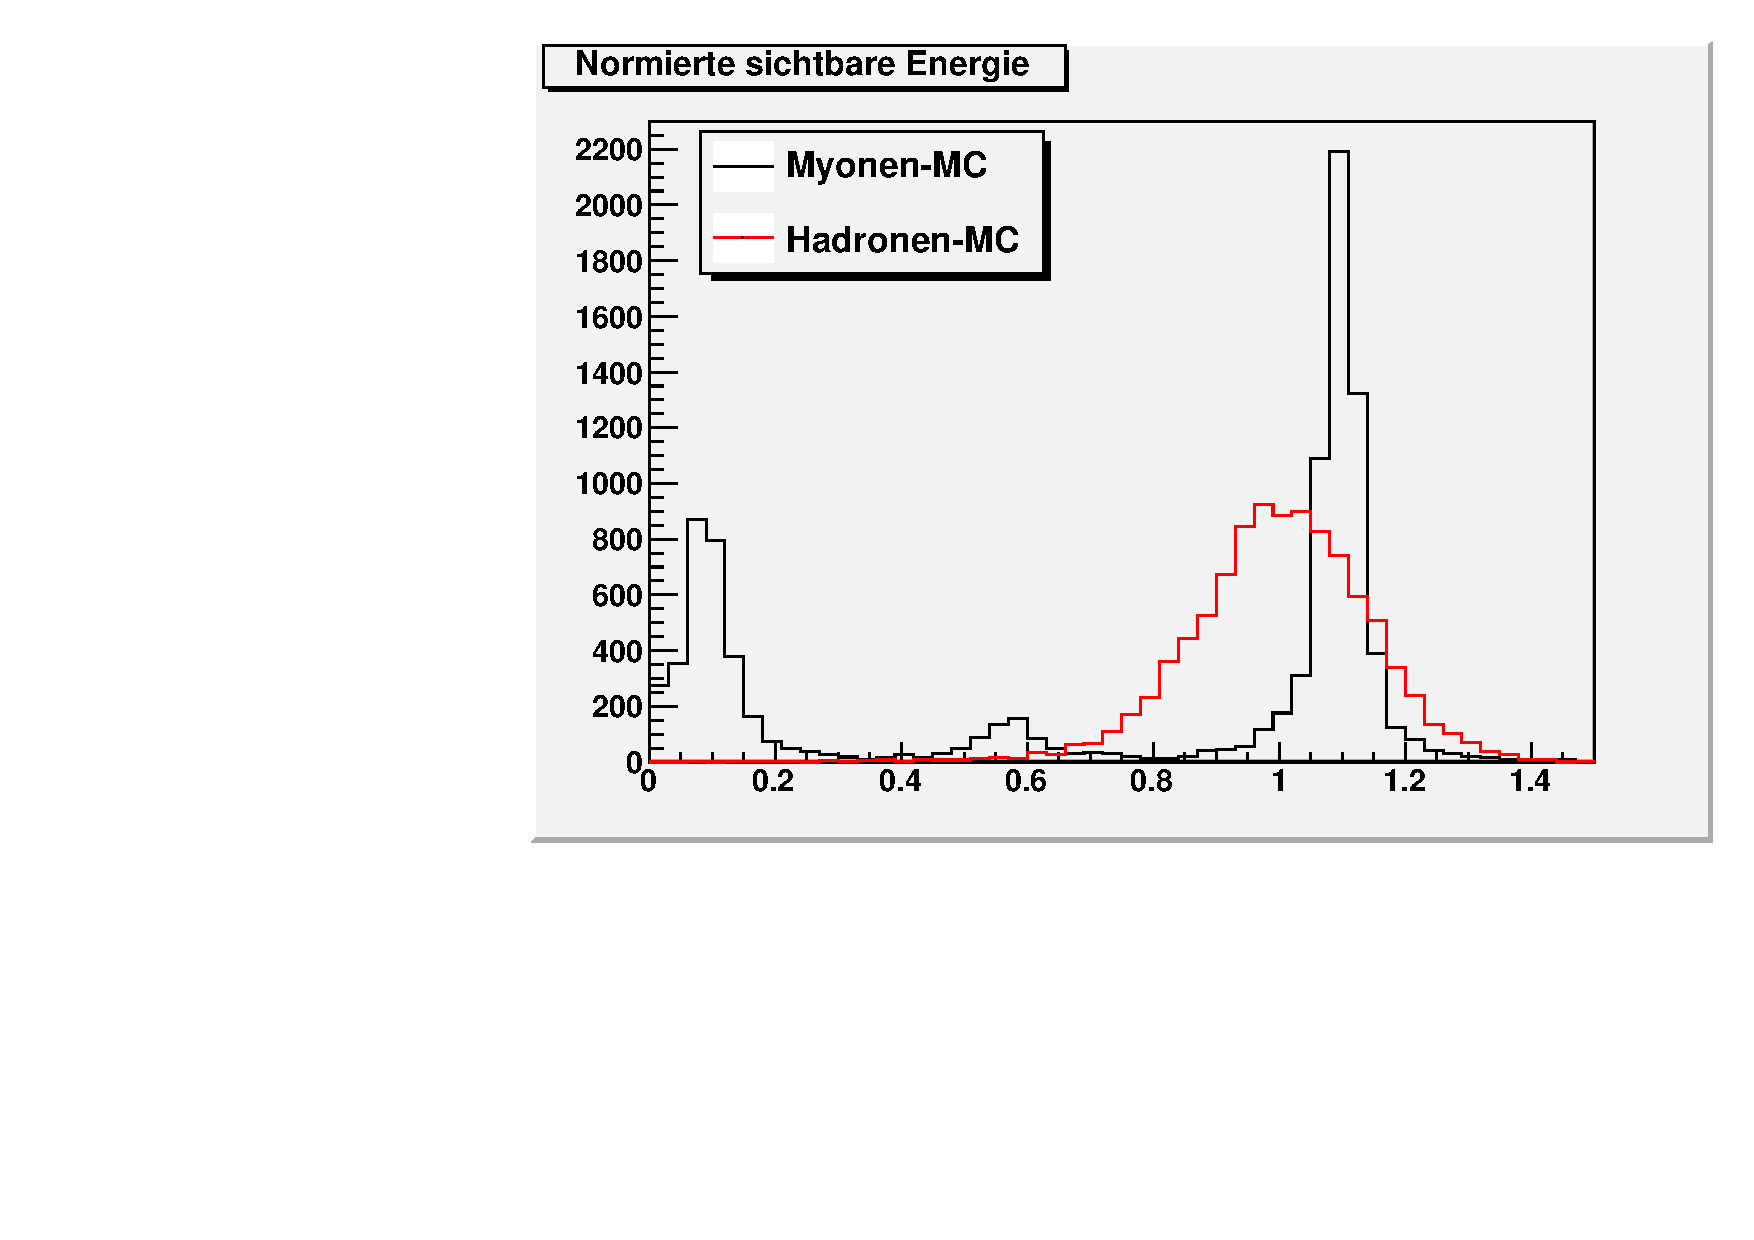
\includegraphics[width=1\columnwidth,keepaspectratio]{Evisvgl_mc.pdf}
	\caption{Verteilung der sichtbaren Energie für MC-Samples}
	\label{fig:Evisvgl_mc}
\end{figure}
Zum Beispiel zerfallen $\tau$-Leptonen oft so, dass die Art und Anzahl der Teilchen, die in die Kalorimeter gelangt, sehr einem hadronischen Ereignis ähnelt. Allerdings wird dabei viel Energie an dabei entstehende Neutrines abgegeben, die nicht registriert werden können, sodass die sichtbare Energie in einem solchen Fall wesentlich kleiner ist. Mit diesem Cut können demnach viele $\tau$-Zerfälle ausgeschlossen werden. Dabei haben wir auch immer darauf geachtet, dass die Effizienz unserer Cuts nicht zu klein wird. Mit den eben erwähnten Cuts gelang es uns, eine Effizienz von
\begin{eqnarray}
\epsilon_\mathrm{Had} &=& \frac{9770 \pm \sqrt{9770} \pm 158}{10000}\\
&=& 0.98 \pm 0.01 \pm 0.02
\end{eqnarray}
zu erreichen. Dabei ist der erste angegebene Fehler der statistische Fehler und der zweite der systematische Fehler, der aus der Variation der Schnittkriterien resultiert. Wenn man diese Cuts allerdings auf das Myonen-Monte-Carlo-Sample anwendet, so werden nur 19 hadronische Events ``gefunden'' (bei 9970 Events im Sample!). Die Fehlerquote durch Myonenereignisse ist also sehr gering. Unsere Schnitte sind also offenbar gut geeignet, um Hadronen-Events aus den Daten zu selektieren.

\subsection{Berechnung der hadronischen Wirkungsquerschnitte bei verschiedenen $\sqrt{s}$}
Die eben besprochenen Schnitte haben wir nun auf die Messdaten angewandt. Dabei kamen die in \tref{hadronic_xsecs} gezeigten Werte heraus. Die angegebenen Fehler sind wiederum statistischer und dann systematischer Fehler. Diese Konvention verwenden wir im gesamten folgenden Protokoll.\\
Der Fehler des Wirkungsquerschnitts ergibt sich durch Fehlerfortpflanzung aus den jeweiligen Fehlern von N und von $\epsilon_\mathrm{Had}$.

\begin{table*}[ht]
\begin{tabular*}{\textwidth}{%
S[tabformat=2.1]%
l%
l}
\toprule
{Energie [\si{GeV}]} &
{Zahl analysierter Hadr.-Ereignisse N} &
{Wirkungsquerschnitt $\sigma_0^{Had}$ [\si{\nano\barn}]}\\
\midrule
89.48 & 1848 ± 43 ± 52 & 10.55 ± 0.18 ± 0.16 \\
91.33 & 3980 ± 63 ± 79 & 29.98 ± 0.49 ± 0.43 \\
93.02 & 2149 ± 46 ± 51 & 14.56 ± 0.24 ± 0.24 \\
\bottomrule
\end{tabular*}
\caption{Zahl der analysierten Hadronen-Ereignisse und zugehörige Wirkungsquerschnitte bei verschiedenen Schwerpunktsenergien}
\label{tab:hadronic_xsecs}
\end{table*}


Der Wirkungsquerschnitt, der auch in \tref{hadronic_xsecs} aufgeführt ist, ergibt sich aus den gegebenen Daten nach \cite[Gl.13]{script} wie folgt:
\begin{eqnarray}
\sigma_\mathrm{Had} = \frac{N - N_U}{L\epsilon_\mathrm{Had}} = \frac{N}{L\epsilon_\mathrm{Had}}
\end{eqnarray}
$N$ ist dabei die Zahl der analysierten Hadronenereignisse, $L$ ist die bereits erwähnte, schwerpunktsenergieabhängige Luminosität und $\epsilon_\mathrm{Had}$ wurde oben bereits eingeführt. Die Zahl der vermuteten Untergrundereignisse $N_U$ haben wir auf null gesetzt, weil unsere Cuts die jeweiligen Events sehr effektiv passieren lassen. Außerdem kann man die Form der Verteilungen von z.B. der sichtbaren Energie (nach den betreffenden Selektionsschnitten) sowohl für die Monte Carlo-Samples wie auch für die Daten-Samples vergleichen (\fref{Evis_vgl}).
\begin{figure}[htb]
	\centering
	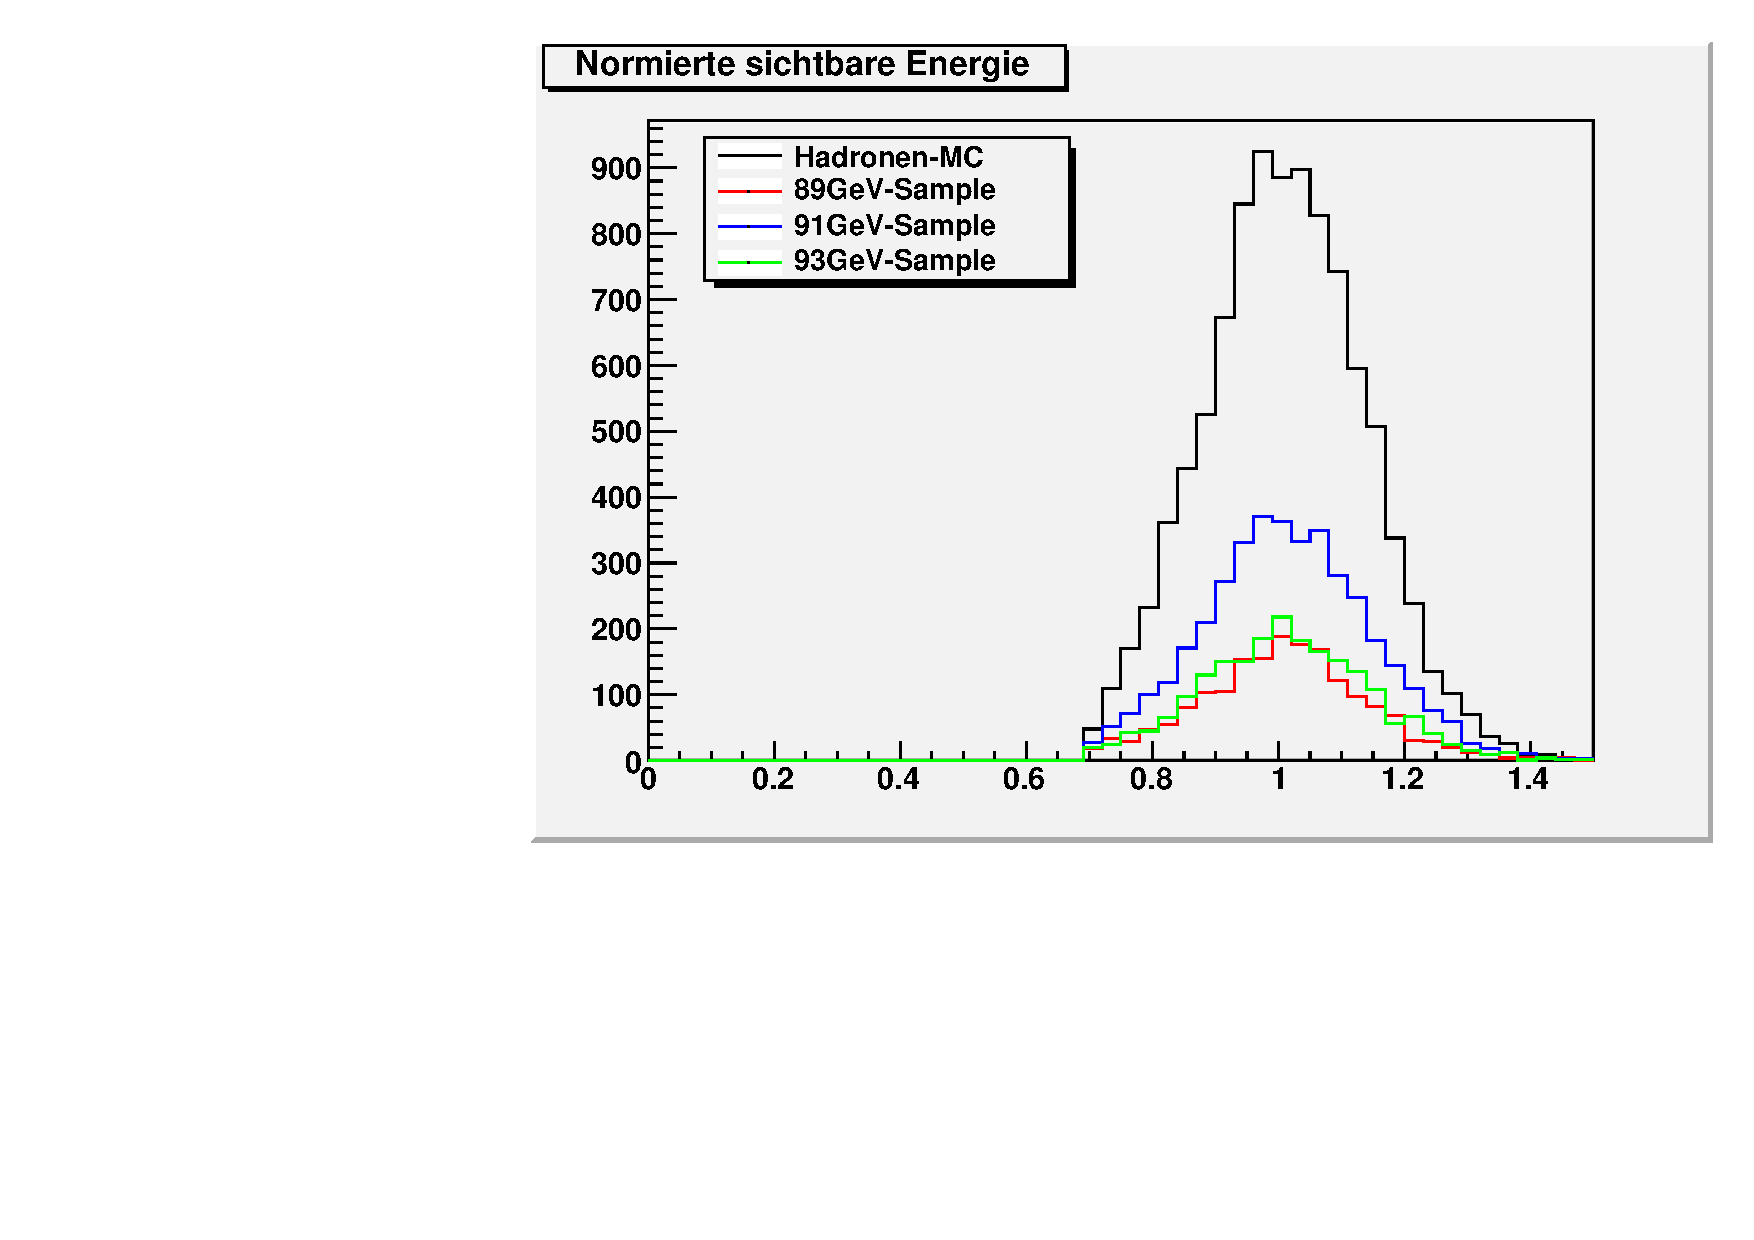
\includegraphics[width=1\columnwidth,keepaspectratio]{Evis_vgl.pdf}
	\caption{Verteilung der sichtbaren Energie für verschiedene Samples}
	\label{fig:Evis_vgl}
\end{figure}
Wie man sehen kann, sehen sich die Verteilungen sehr ähnlich, was die Vermutung nahelegt, dass vornehmlich die gleichen Prozesse stattfanden. Dies bestätigt uns in der Annahme, dass der Untergrund mit gutem Gewissen vernachlässigt werden kann.\\
Der statistische Fehler des Wirkungsquerschnitts ergibt sich durch Fehlerfortpflanzung aus den jeweiligen Fehlern von $N$, $L$ und $\epsilon_\mathrm{Had}$:
\begin{equation}
  \begin{split}
    \Delta\sigma_\mathrm{Had} =  \sqrt{\left( \frac{\partial\sigma}{\partial L}\Delta L\right)^2 + \left( \frac{\partial\sigma}{\partial N}\Delta N\right)^2} \\
    \overline{+ \left( \frac{\partial\sigma}{\partial \epsilon_\mathrm{Had}}\Delta\epsilon_\mathrm{Had} \right)^2} \\
    = \sqrt{\left( \frac{N}{L^2\epsilon_\mathrm{Had}}\Delta L\right)^2 + \left( \frac{1}{L\epsilon_\mathrm{Had}}\Delta N\right)^2} \\
    \overline{+ \left( \frac{N}{L \epsilon_\mathrm{Had}^2}\Delta\epsilon_\mathrm{Had} \right)^2}
  \end{split}
\end{equation}

In dieser Art haben wir auch alle weiteren Fehler berechnet, wie z.B. den systematischen Fehler von $\sigma_\mathrm{Had}$, der sich aus den systematischen Unsicherheiten von $N$ und $\epsilon_{\mathrm{Had}}$ zusammensetzt.

Diese Wirkungsquerschnitte kann man nun in das bereitgestellte Fit-Programm einsetzen. Dieses Programm wurde von uns leicht verändert und kann im Anhang A unter \lref{fit} gefunden werden. Es resultierte der Fit in \fref{hadfit}.\\
\begin{figure}[htb]
	\centering
	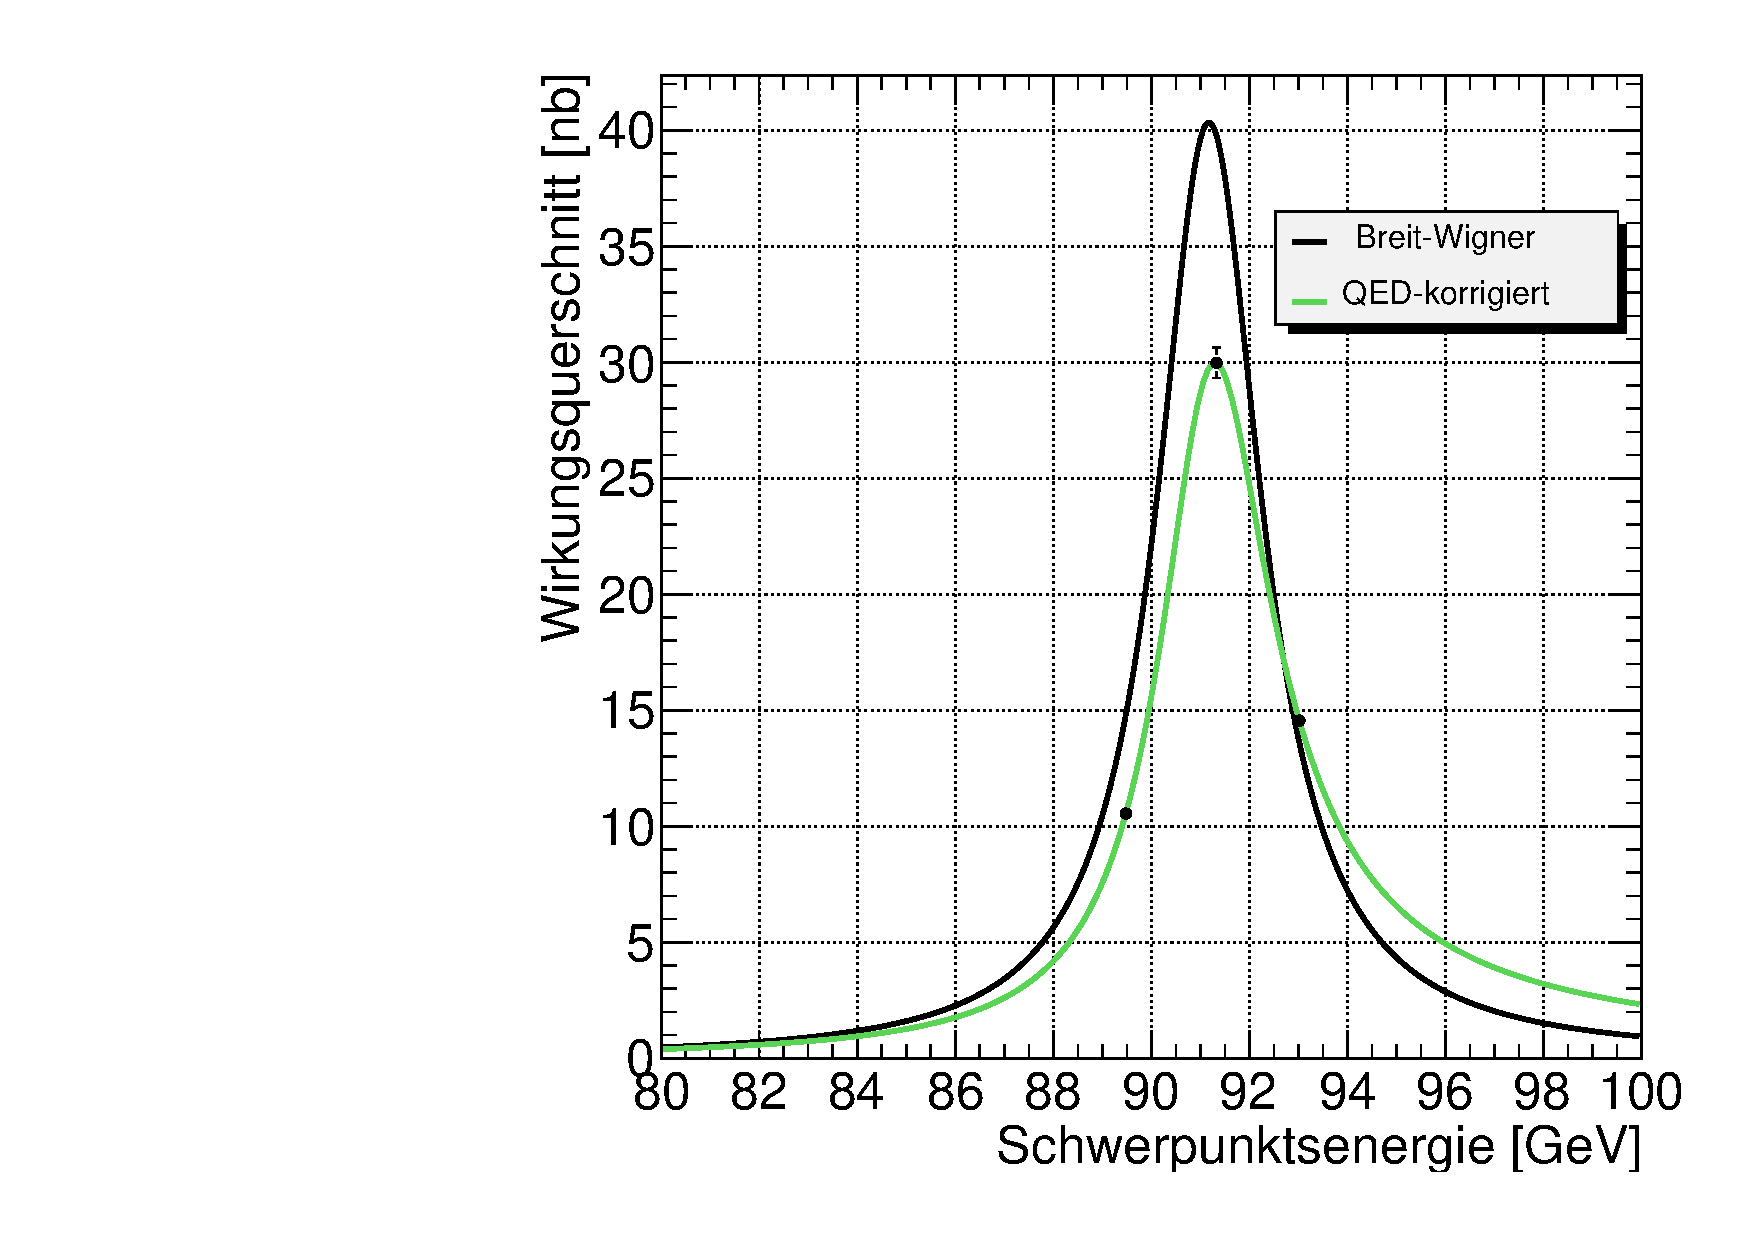
\includegraphics[width=1\columnwidth,keepaspectratio]{fit_had}
	\caption{Fit des hadronischen Wirkungsquerschnitts in Abhängigkeit von $\sqrt{s}$}
	\label{fig:hadfit}
\end{figure}
Unter Berücksichtigung der statistischen Fehler von N, $\epsilon_\mathrm{Had}$ und der Luminosität (deren Fehler war in \cite[S.9]{script} mit $1\%$ des gegebenen Wertes angegeben) kann der statistische Fehler von $\sigma_0$ und mit den systematischen Fehlern von N und $\epsilon_{\mathrm{Had}}$ durch dieses Programm berechnet werden. Für den gesamten hadronischen Wirkungsquerschnitt resultiert also:
\begin{equation}
\sigma_0^{\mathrm{Had}} = (40.33 \pm 0.65 \pm 0.27) \si{\nano\barn}
\end{equation}

Der Gesamtfehler, der pythagoräisch aus dem systematischen und dem statistischen Fehler addiert wird, beträgt mit $0.7\si{\nano\barn}$ ungefähr $2\%$ des Absolutwertes.\\
Der $\chi^2$-Wert der Anpassung war mit $8\cdot10^{-12}$ sehr klein, allerdings interessiert meist eher der Wert $\chi^2/$DoF, wobei DoF die ``Degrees of Freedom'', also die Anzahl der Freiheitsgrade, ist. Dieser Wert sollte nahe null liegen. Da in diesem Fall aber drei Parameter festgelegt werden mussten, wofür nur drei Messpunkte zur Verfügung standen, ist DoF gleich null. Daher ist unbestimmt, wie groß der $\chi^2/$DoF-Wert nun eigentlich ist. Auf jeden Fall kann man dem Plot \fref{hadfit} ansehen, dass der Fit gut durch die Datenpunkte verläuft. Man kann den Parametern also Glauben schenken, auch ohne genaue Kenntnis über $\chi^2/$DoF.\\
Weiterhin konnte man der Breit-Wigner-Anpassung auch die Werte für die Zerfallsbreite $\Gamma_Z$ und für die Masse $M_Z$ entnehmen:
\begin{eqnarray}
\Gamma_Z &=& (2.61 \pm 0.05 \pm 0.03)\si{\giga\electronvolt}\\
M_Z &=& (91.16 \pm 0.02 \pm 0.02)\si{\giga\electronvolt}
\end{eqnarray}
Aus der Zerfallsbreite kann man die Lebensdauer des $Z^0$ berechnen:
\begin{eqnarray}
\tau_Z &=& \frac{1}{\Gamma_Z}\\
&=& (2.53 \pm 0.31 \pm 0.02)\cdot 10^{-25}\si{\second}
\end{eqnarray}
Die Ergebnisse werden im Kapitel 5 ``Diskussion der Ergebnisse'' auf ihre Übereinstimmung mit Literaturwerten überprüft.

\section{Bestimmung des myonischen Wirkungsquerschnitts $\sigma_0^{\mu}$}
\subsection{Selektion der Myonenereignisse}
Hier wurde genauso wie bei der Selektion der Hadronenevents vorgegangen. Wie bereits oben in \fref{Ncluster_vgl} gezeigt, haben alle Myonen-Ereignisse weniger als 12 Cluster-Einträge,
so dass hier ein Cut gesetzt werden konnte. Weiterhin kann man verlangen, dass mindestens zwei Teilchen die Masse eines Myons besitzen müssen. Außerdem muss der Betrag des Kosinus' des Winkels, den die Bahnen beider Myonen bilden, größer als 0.9 sein, womit man fordert, dass die Myonen annähernd Back-to-Back fliegen. Schließlich wurden an die Energie eines Events einige Anforderungen gestellt.
Das Teilchen mit der meisten Energie soll ungefähr die Hälfte der sichtbaren Energie des gesamten Events tragen. Darüber hinaus soll die gemessene (sichtbare) Energie relativ zur Schwerpunktsenergie im Intervall von \SI{80}{\percent} bis \SI{140}{\percent} liegen. Die Tatsache, dass auch Events mit mehr als \si{100}{\percent} gemessen wurde, zeigt, dass die Energiemessung des Detektors offenbar mit größeren Fehlern behaftet ist.
Inspiriert wurden diese Cuts im Wesentlichen durch \cite[Kap. 5]{kap5}. Mit diesen Schnitten wird eine Effizienz von
\begin{equation}
  \begin{split}
    \epsilon_{\mathrm{Mu}} &= \frac{5855 \pm \sqrt{5855} \pm 197}{9970} \\ &= 0,59 \pm 0,01 \pm 0,02
  \end{split}
\end{equation}
erreicht. Nun können, analog zum Hadronen-Fall, die Wirkungsquerschnitte bei den verschiedenen Schwerpunktsenergien angegeben werden. Die Ergebnisse sind in \tref{muonic_xsecs} zu finden.
\begin{table*}[ht]
\begin{tabular*}{\textwidth}{%
S[tabformat=2.1]%
l%
l}
\toprule
{Energie [\si{GeV}]} &
{Zahl analysierter Myonen-Ereignisse N} &
{Wirkungsquerschnitt $\sigma_0^{\mu}$ [\si{\nano\barn}]}\\
\midrule
89.48 & 67 ± 8 ± 8  & 0.64 ± 0.03 ± 0.3 \\
91.33 & 122 ± 11 ± 10 & 1.53 ± 0.05 ± 0.4 \\
93.02 & 77 ± 9 ± 9 & 0.87 ± 0.04 ± 0.03 \\
\bottomrule
\end{tabular*}
\caption{Zahl der analysierten Myonen-Ereignisse und zugehörige Wirkungsquerschnitte bei verschiedenen Schwerpunktsenergien}
\label{tab:muonic_xsecs}
\end{table*}

\subsection{Bestimmung des Wirkungsquerschnitts}
Mit den in \tref{muonic_xsecs} aufgelisteten $\sqrt{s}$-abhängigen Wirkungsquerschnitten kann man nun wiederum das Fit-Programm aufrufen. Dabei sollte einzig $\sigma_0$ angepasst werden, während die totale Zerfallsbreite des $Z^0$ und die Masse $M_Z$ als feste Parameter, die aus der hadronischen Anpassung resultierten, übergeben wurden. Das Fit-Ergebnis (in \fref{muonfit} zu sehen) lautet also:
\begin{eqnarray}
\sigma_0^{\mu} = (2.16 \pm 0.05 \pm 0.03)\si{\nano\barn}
\end{eqnarray}
\begin{figure}[htb]
	\centering
	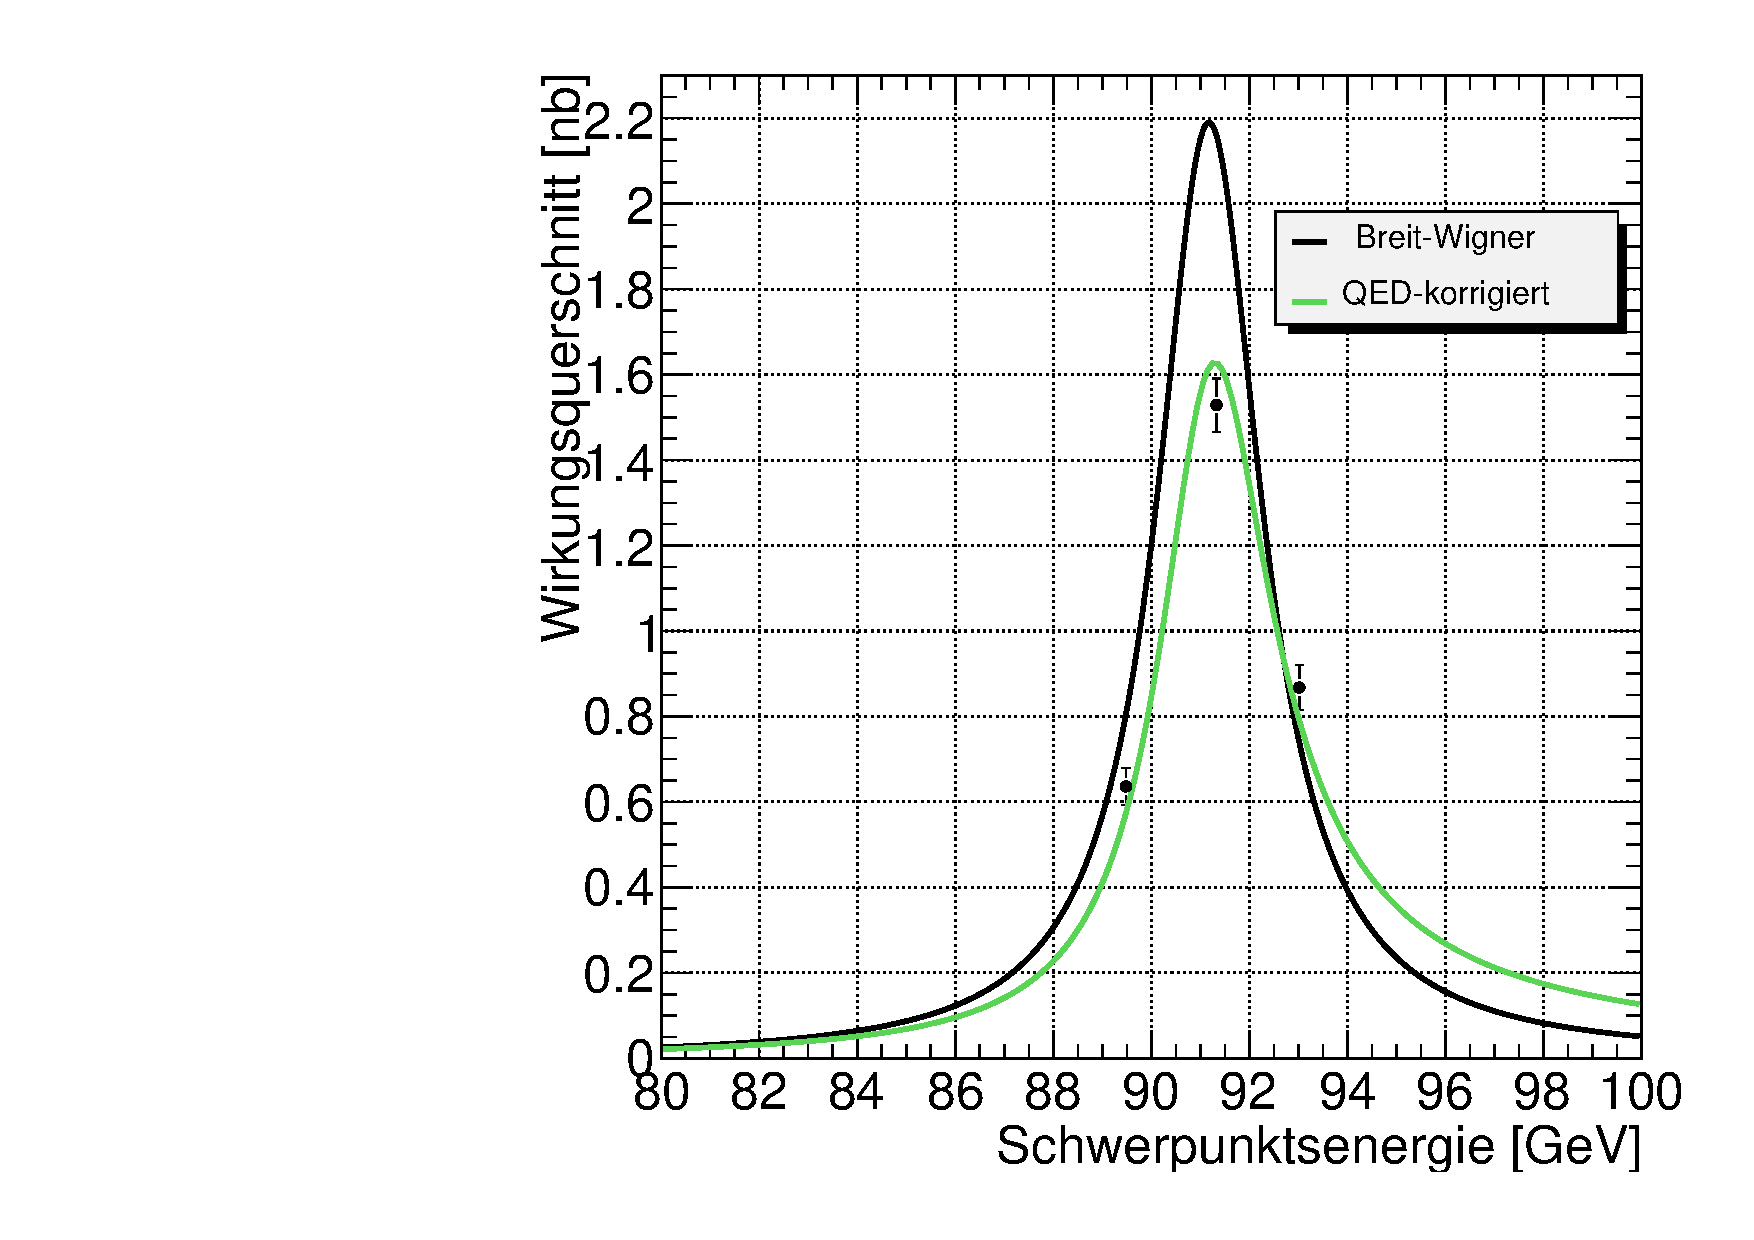
\includegraphics[width=1\columnwidth,keepaspectratio]{fit_muon}
	\caption{Fit des myonischen Wirkungsquerschnitts in Abhängigkeit von $\sqrt{s}$}
	\label{fig:muonfit}
\end{figure}
Der myonische Wirkungsquerschnitt ist also deutlich kleiner als der hadronische.\\
Der $\chi^2/$DoF-Wert kann hier genau angegeben werden, da in diesem Fit nur ein einziger Parameter variiert werden musste und DoF somit gleich zwei ist. $\chi^2/$DoF beträgt in diesem Fall also 3.4, was schon in der richtigen Größenordnung liegt.

\section{Bestimmung einiger Partialbreiten, des Weinbergwinkels und des Farbfaktors}
\subsection{$\Gamma_e$-Bestimmung}
\subsubsection{$\Gamma_e$-Bestimmung aus dem myonischen Wirkungsquerschnitt}
Man kann die elektronische Partialbreite aus \cite[Gl.5]{script} bestimmen:
\begin{eqnarray}
 \sigma_0 &=& \frac{12\pi}{M_Z^2}\frac{\Gamma_e\Gamma_f}{\Gamma_Z^2}
\end{eqnarray}
Wenn man nun als aus dem $Z^0$-Zerfall entstehendes Teilchen ein Myon einsetzt, so wird aus $\Gamma_f\rightarrow\Gamma_{\mu}$, und als Wirkungsquerschnitt wird dann $\sigma_0^{\mu}$ eingesetzt.
\begin{eqnarray}
\sigma_0^{\mu} &=& \frac{12\pi}{M_Z^2}\frac{\Gamma_e\Gamma_{\mu}}{\Gamma_Z^2}\\
 \Gamma_e &=& \Gamma_{\mu} = \Gamma_{tau}\\
 \rightarrow \Gamma_e &=& \sqrt{\frac{M_Z^2\sigma_0^{\mu}}{12\pi}}\Gamma_Z\\
 &=& (91 \pm 2 \pm 1)\si{\mega\electronvolt}
\end{eqnarray}
Dabei wurde die Beziehung \cite[Gl.9]{script} verwendet, sodass man statt der myonischen genausogut die elektronische Zerfallsbreite berechnen kann.\\
Weiterhin konnte man die elektronische Zerfallsbreite auch mit der folgenden Methode bestimmen:
\begin{eqnarray}
\Gamma_e &=& \frac{1}{3}(\Gamma_Z - 3\Gamma_{Had} - 3\Gamma_{\nu_l})\\
\Gamma_{Had} &=& \frac{M_Z^2\Gamma_Z^2\sigma_0^{Had}}{12\pi}\cdot\frac{1}{\Gamma_e}\\
&=& \frac{\alpha}{\Gamma_e}\\
\Gamma_{\nu_e} &=& \frac{G_FM_Z^3}{12\sqrt{2}\pi}\\
&=& (165.71 \pm 0.10 \pm 0.09)\si{\mega\electronvolt}\\
\beta &=& \frac{1}{3}\Gamma_Z - \Gamma_{\nu_e}\\
0 &=& \Gamma_e^2 - \beta\Gamma_e + \alpha\\
\Gamma_{e,1} &=& 0.61\si{\giga\electronvolt}\\
\Gamma_{e,2} &=& 0.083\si{\giga\electronvolt}\\
\rightarrow \Gamma_e &=& \Gamma_{e,2}\\
&=& (83 \pm 4 \pm 3) \si{\mega\electronvolt}
\end{eqnarray}
Da dies die Lösung einer quadratischen Gleichung ist, muss man sehen, welche der beiden Lösungen die physikalisch sinnvollere ist. In diesem Fall haben wir die Lösung gewählt, die besser mit der vorher berechneten elektronischen Partialbreite übereinstimmt. Diese beiden Zerfallsbreiten stimmen also sehr gut überein (die relative Abweichung beträgt nur knapp 9\si{\percent}, und die Fehlerbereiche überschneiden sich).

\subsection{Bestimmung des Weinbergwinkels}
Aus den bisher bekannten Größen kann man über die in \cite[Gl.6]{script} gegebene Formel den Weinbergwinkel berechnen. Wir verwenden hierfür die eben (mit der zweiten Methode) bestimmte elektronische Partialbreite des $Z^0$-Zerfalls.
\begin{eqnarray}
\Gamma_e &=& \frac{G_F M_Z^3}{24 \sqrt{2}\pi}\left(1+[1-4|Q_e|\sin^2\Theta_W]^2\right)\\
|Q_e| &=& 1
\end{eqnarray}
Damit folgt also für die den Weinbergwinkel:
\begin{eqnarray}
\sin^2\Theta_W &=& \frac{1-\sqrt{\frac{\Gamma_e\cdot 24\sqrt{2}\pi}{G_FM_Z^3}-1}}{4}\\
&=& 0.23 \pm 0.05 \pm 0.08\\
\Theta_W &=& \arcsin(\sqrt{\sin^2\Theta_W})\\
&=& 0.50 \pm 0.11 \pm 0.07\\
&=& (28 \pm 6 \pm 4)\symbol{23}
\end{eqnarray}
Dabei muss man beachten, dass das Ergebnis der Rechnung imaginär ist. Wir haben aber nur den physikalischen Anteil, also den Realteil des Ergebnisses, als Weinbergwinkel verwendet. Für den Vergleich mit den Literaturwerten verweise ich wiederum auf \cite[Kap. 5]{kap5}.

\subsection{Bestimmung der hadronischen Partialbreite}
Aus den bereits bekannten Partialbreiten für die geladenen und ungeladenen Leptonen lässt sich nun auch noch die hadronische Partialbreite nach \cite[Gl.8]{script} berechnen:
\begin{eqnarray}
\Gamma_Z &=& \Gamma_{had} + 3\Gamma_{\nu_e} + 3\Gamma_e\\
\Gamma_{Had} &=& \Gamma_Z - 3\Gamma_{\nu_e} - 3\Gamma_e\\
&=& (1.86 \pm 0.05 \pm 0.03)\si{\giga\electronvolt}
\end{eqnarray}

\subsection{Bestimmung des Farbfaktors}
Abschließend konnten wir noch den Farbfaktor $N_C$ berechnen, indem wir \cite[Gl.15]{script} verwendeten:
\begin{eqnarray}
\Gamma_{Had} &=& N_CK_{QCD}(2\Gamma_u + 3\Gamma_d)
\end{eqnarray}
$\Gamma_u$ und $\Gamma_d$ berechnen wir mit Hilfe der bereits eingeführten Formel \cite[Gl.6]{script}, wobei für die Ladungen der Quarks die Werte $\frac{2}{3}$ für das Up-Quark und $-\frac{1}{3}$ für das Down-Quark eingesetzt wurde. Damit folgt für $N_C$:
\begin{eqnarray}
N_C &=& \frac{\Gamma_{Had}}{K_{QCD}(2\Gamma_u + 3\Gamma_d)}\\
&=& 3.20 \pm 0.11 \pm 0.07
\end{eqnarray}
Dieses Ergebnis legt also den Schluss nahe, dass es die bereits bekannten drei Quarkfamilien gibt (Up-Down, Charm-Strange, Top-Bottom).